\chapter{BGP state of the art}
\label{cha:bgp_art}

\ac{BGP} is the protocol used to control the information spreading on the Internet.
It is at the version \num{4} published in \num{2006} with the \ac{RFC} \num{4271}
\cite{rfc4271}.
\ac{BGP} is a \ac{PV} protocol, it distinguish itself from the \ac{DV} and \ac{LS}
protocols with the major difference that it shares other than the knowledge of
a path also the path itself to reach the destination.

\ac{BGP} has two major sub-cateogies with a difference in the flow of information
direction:
\begin{itemize}
	\item \textbf{\textit{\ac{eBGP}}}, we talk about \ac{eBGP} when the
		flow of information goes from the inside
		of the \ac{AS} to other \acp{AS};
	\item \textbf{\textit{\ac{iBGP}}}, we talk about \ac{iBGP} when the flow
		of information goes from the outside of the \ac{AS} to the inside of
		it, to make aware of the new route also the internal routing protocol.
\end{itemize}

My main interest in this thesis is for the \ac{eBGP} part of the protocol, for
now on I will refer to it talink in general of \ac{BGP} without further distinguish
from the internal protocol.

When there is an interconnection between two \acp{AS} that creates a \ac{BGP}
link, I will talk about peering refering to thi connection, and those \ac{BGP} 
speakers interconnected will be the peers.
Each \ac{BGP} connection is based on a direct \ac{TCP} connection.
On this links every \ac{AS} can configure its own policies that would be used
to evaluate routes at the reception or at the output \fxfatal{Find a better word}.
There are three different possible type of relations that can be created by two
\ac{BGP} speaker, accordingly to the \ac{CAIDA}:

\begin{itemize}
	\item \textbf{\textit{\ac{c2p}}} This relationship higlights the fact that
		lower \ac{AS} pays a hiher level \ac{AS} to get connectivity and access
		to the Ineternet;
	\item \textbf{\textit{\ac{p2p}}} This relationship is used to share the knowledge
		between two \acp{AS} of their customer providers without paying a higher
		level \ac{AS};
	\item \textbf{\textit{\ac{s2s}}} This relationship defines the connection 
		between \acp{AS} under the same \ac{ISP}.
\end{itemize}

During this thesis I will only consider the first two relationships \ac{c2p} and
\ac{p2p}, the schema in \fxfatal{Insert figure} shows how the traffic is affected
based on the type of the link crossed.

As showed by the flows with a different color in \fxfatal{insert figure} a single
\ac{AS} will share information considering the receiving link.
If something cames from one of its customers it will share the knowledge with
every other link that it has (always respecting the output policies).
If a route has come from its provider or a peer then it will be only shared with 
its own customers.
Those policies are dictated by convenience, an \ac{AS} has all the advantages when
other \acp{AS} decide to use it to reach a specific destination.

This behaviour can be modeled with a variant of the \ac{SSP} algebra described
in \cite{daggitt2018rate}.
This is the same algebra that will be used in \Cref{cha:des} to describe link
relationships.

%\begin{itemize}
%    \item BGP de facto standard on the internet
%    \item What is an AS
%    \item interconnection between ASes
%\end{itemize}

\section{BGP}
\label{sec:bgp_intro}

Once a \ac{BGP} node has estabilished a connection with an other peer it will
start to exchange routes with that neighbour, always respecting the policies.

Every \ac{BGP} nodes has a \ac{RIB} as data structure to keep the information
about the received routes, the alternative routes and what should be exported.
The \ac{RIB} is divided into \num{3} sections.
\begin{itemize}
	\item \textbf{\textit{ADJ-RIB\_in}} This \ac{RIB} contains all the routes
		that have been received by other \ac{AS} in order to be evaluated;
	\item \textbf{\textit{LOC-RIB}} This \ac{RIB} contains all the best routes
		that have been chosen from the \textit{ADJ-RIB\_in} from the node;
	\item \textbf{\textit{ADJ-RIB\_out}} There is an output \ac{RIB} for every
		neighbour of the node, it contains the route that should be advertised 
		to the specific node.
\end{itemize}

One of the most important part of \ac{BGP} is its decision process, that would
be applyed to discern between the routes in the \textit{ADJ-RIB\_in} in order
to update the \textit{LOC-RIB} and, if necessary also the \textit{ADJ-RIB\_out}.
The decision process is composed by three parts:
\begin{itemize}
	\item[1] Calculation of the preference: This function is called every time
		there are new rechability information that needs to be evaluated, it 
		will assign/update the preference value at every route in the 
		\textit{ADJ-RIB\_in} using policy filters preconfigured. If a route
		doesn't respect the policy filters it will be then marked as ineligeble,
		otherwise a \textit{PREF\_VALUE} will be calculated and assigned to the
		route.
	\item[2] Route selection: This function is called at the end of the first
		phase, it collects all the eligeble routes and evaluate them removing
		routes that would create loops or that creates conflicting situations.
		The evaluated routes are then ordered by the \textit{PREF\_VALUE} and
		then the best route will be then installed in the \textit{LOC-RIB}.
		In case of ties there is an algorithm that can be used to break them.
	\item[3] Route dissemination: This function can be called in different
		situations, it will use the information in the \textit{LOC-RIB} to
		populate every \textit{ADJ-RIB\_out}, according to configuration
		policy.
\end{itemize}
The decision process is also responsible for the route aggregation and information
reduction.
At the end of the third phase the \ac{BGP} speaker will execute the
\textit{Update-send} process, that is responsible for the effective dissemination.

There are multiple types of packets that can be sent by a \ac{BGP} speaker, but
we will focus only on the \ac{ADV} packets.
The \ac{ADV} packets are responsible for the dissemination of the information
to other nodes that will analyze and use the attribute inside the message
to assign a preference value to the route.
In particular there are two section of the \ac{ADV} messages that will 
contain additive information and subtractive information.
We can distinguish \ac{ADV} messages using the type of information that are 
transmitting:
\begin{itemize}
	\item \textbf{\textit{UPDATE}}, this type of messages represent the distribution
		of new reachability information, a new route to a destination will be
		shared through an update message;
	\item \textbf{\textit{WITHDRAW}}, this type of messages are distributed when
		a node want to share that it doesn't know how to reach a destination
		a destination anymore.
\end{itemize}
Inside those packets there are different attributes that permit to transfer 
information about the route (advertised or withdrawd).
There is an attribute that describe the address that the route represents,
another one that contains the path that will be used to reach the 
destination, the next hop used, etc.
During the year multiple new \ac{RFC} have introduced, modified, updated, removed
attributes that can be found inside an advertisemente message.
Not all the attributes are mandatory for \ac{BGP} nodes, infact for a node
is possible to receive a route with attribute that it is not able to interpret
but (if configured to do so) it will share the route with also the unknown 
attributes.

Is important to remember that all those information are useful for the policy
filter that every node can have, for example some nodes would automatically discard
any route that contains a specifi \ac{AS} in the received path.

The \textit{Update-send} process is responsible for the distribution of the 
messages that are stored in the \textit{ADJ-RIB\_out}.
It should execute again some checks on the \ac{RIB}, removing unfeasible routes
and remving routes that has already been advertised to the pear.
It also has to respect a temportal constraint, introduced in \cite{rfc4271}, 
a \ac{BGP} speaker can't send to the same neighbour routes for the same destination
more often than the \ac{MRAI} value.
\ac{MRAI} act as a timer which goal is to avoid continous update storm caused
by decision changes in some peers in the network.

Another property that can be found in \ac{BGP} nodes that affects the messages
transmitted is the \ac{IW}.
This property permits to reduce the number of messages tha are distributed.
Without this option when a \ac{BGP} node discover a new besth path to reach
a destination should send a withdraw followed by an update to its neighbourhood.
Thanks to this option is sufficient to send just the update, the other nodes 
will learn that the best path is changed simply looking to the previous 
alternative and comparing them.

%\begin{itemize}
%    \item High level of BGP
%    \item BGP messages
%    \item BGP Update messages
%    \item BGP policies
%	\item two type of BGP noise, the one caused by BGP itself and the one 
%		caused by flapping interfaces
%\end{itemize}

%\section{BGP Wedgies}
%\label{sec:bgp_wedgies}
%
%\begin{itemize}
%    \item What are wedgies?
%    \item why are them important?
%    \item which situations them occur?
%\end{itemize}

\section{BGP Noise}
\label{sec:bgp_noise}

There are basically two type of noises in \ac{BGP}, the inherent noise and the 
noise caused by external sources.
Those two type of noises are triggered by different causes but are substantially
not discernible one another.

The first one is caused by the protocol itself when it tryies to convergence 
on new knowledge.
The sharing of new routes can cause new \ac{ADV} that can then trigger the
\textit{Path Exploration} problem.
This is a noise caused by the protocol itself that acts as eco chamber for 
new best paths that changes untill the best possible path is taken in consideration.

One \ac{BGP} parameter tries to limit this noise acting as a message chache with
a compression system.
This parameter is \ac{MRAI} and it permits to avoid sending a message for every
new one received using a timer.
Only the best decision after that time will be shared.

The second type of noise is caused by a source outside the protocol.
A missconfiguration, a faulty interface can cause the send of not necessary messages.
For example the withdraw and the advertisement of a route at continous intervarl.
This type of behaviour will cause continuous storms of messages and the triggering
of the first noise type.

\ac{BGP} introduce a parameter with the \ac{RFC} \num{2439} \cite{rfc2439} that
is called \ac{RFD} to overcome this behaviour.
This paramter increases a value every time a flap or a route change are detected,
when this value passes a predefined threshold the route will be suppressed.
This value will alway decay using an exponential decay function, even if it 
doesn't overpass the threshold.
Once the route has been suppressed the \ac{BGP} speaker must wait enough time
that the value goes below an other threshold before sharing it again.

Those two parameters are clearly correlated one another from the fact that
one triggers the other and vice versa, is possible to create particular topology
that has different performances based on the values assigned to those 
parameters.
Think about two clique networks connected one another by only one node, this
node will act as a bottleneck, probably its \ac{RFD} threshold would be easily
overpassed and then it depends on it decay function before it can send
again the network to the second clique triggering \ac{MRAI} on those nodes that
will experience the path exploration problem.

\fxfatal{I think that the graphs in Fig 2 and Fig 3 of Fabrikant et al. in 
\cite{fabrikant2011there} will easily trigger both \ac{MRAI} and \ac{RFD}}
\section{BGP MRAI}
\label{sec:bgp_mrai}

\ac{MRAI} is one of the parameters that mostly affect the convergence of \ac{BGP}
A high value of it could unnecesarly delay the transmission of messages, but
in the opposite case a value too small can provoke a lot of messages, one for
every decision change of the node.
There are a lot of studies about it, and it has already been showed that
the number of messages and the convergence of time can depend on it \cite{griffin2001experimental}.
It has been also already proven by Fabrikant, Rexford et al. \cite{fabrikant2011there} 
that an incorrect configuration of it could lead to tremendous consequences.

\ac{MRAI} has been introduced in the \num{4}th version of \ac{BGP} \cite{rfc4271} and
it is nowadays a mandatory argument for every \ac{BGP} node, otherwise the load
in terms of messages to process and decision changes would be incalculable.
Its main purpose, as anticipated in \Cref{sec:bgp_noise} is to prevent, or
at least mitigate the noise created by \ac{BGP} itself.

At the base of \ac{MRAI} there is a timer that controls how much time must pass
between one \ac{ADV} and the following one.
The timer is peer-based, for each interconnection an \ac{AS} could have a different
\ac{MRAI}, but it acts for every destination in parallel, this means that there 
is a different timer for each destination that a node would share for every 
\ac{BGP} relations that it has.
The idea behind it is taht in this time the \ac{BGP} node will be able
to receive other possible routes, evaluate them and send a decision on the 
best route considering multiple alternatives.
It has the property to compress the input messages sequence in order to have
an output message sequence with a smaller number of \ac{ADV}.

The use of \ac{MRAI} is as follow every time the route selection proces change
a route in the \textit{OUT} \ac{RIB} of a neighbour:
\begin{itemize}
	\item If there isn't an active \ac{MRAI} timer for the destination change
		send the \ac{ADV} and set an \ac{MRAI} timer.
	\item If there is an active \ac{MRAI} timer for the destination then 
		don't send anything.
	\item When the active \ac{MRAI} timer ends if there still is the necessity
		to send an \ac{ADV} the send it and set an other \ac{MRAI} timer.
\end{itemize}

The second passage permits to the route selection process to be executed multiple
times before the actual transmission of the decision.
Thats because \ac{MRAI} limits only the transmission and not the decsion process.
The condition to the last passage is due to the fact that the compression some
times could lead to the unnecessity to actually send a message.

The default value defined in the \ac{RFC} \num{4271} for \ac{MRAI} is equal to
\SI{30}{\second}.
But, \ac{MRAI} is a really controversial parameter, it has received multiple
revesions and studies.
In \num{2008} there has been a proposal to reset it default value to \SI{5}{\second}
\cite{jakma2008revised} thanks to different studies that takes in consideration
the dimension of the topology and the latency \cite{qiu2005optimal}.
In \num{2010} a proposal \ac{RFC} of \textit{IETF} \cite{jakma2010revisions} 
says that the default would be left to the arbitrary choice of the operators and
that withdraw message could compleatly avoid it.
But this freedom would damage the convergence and the number of messages distributed
as shoed by Fabrikant et al. \cite{fabrikant2011there}.

Is clear that \ac{MRAI} affect the network performances, but what affects \ac{MRAI}
and, by consequences, the performances?
Obviously the choice itself of a different \ac{MRAI} strategy, as showed for 
example in \cite{milani2019BGP} where the centality was used to obtain better
results in case of network faults.
But, giving the fact that the main function of \ac{MRAI} is to compress the 
input messages also the sequence of messages recept could be meaningful.
Giving that \ac{MRAI} is a link-based parmeters also the number of links that
a node has could influence it, and by consequences the position in the topology.
A well connected node will be more likely to receive multiple paths and messages
than one with only one link.

%\begin{itemize}
%    \item What is MRAI?
%	\item Rember that the MRAI purpose is to avoid the BGP noise
%    \item Previous works on MRAI
%    \item Suppositions on the MRAI influence
%\end{itemize}

\section{BGP RFD}
\label{sec:bgp_rfd}

\ac{RFD} is a parameter introduced in \ac{BGP} to overcome the problems caused
by the exterior sources of noise.
Its main function is to avoid fluctuating routes to overload \ac{BGP} nodes 
with continous message storms.
It has been introduced with the \ac{RFC} \num{2439} in \num{1998} \cite{rfc2439}.
Also \ac{RFD} is a controversial parameter, it has been studied and revaluated
different times, but recent studies showed that the majority of the operators 
still use deprecated values from \num{2001} \cite{gray2020bgp}.
Furthermore, other studies shows that the majority of the \ac{ADV} that thravels
through the Internet are genereated by a restricted set of \ac{AS} but \ac{RFD}
seems to be to restrictive and affect the majority of the \acp{AS} traffic
\cite{pelsser2011route}.

\ac{RFD} will use a single value, called \textit{figure of merit}, to evaluate
the actual situation of a route, while this value evolve the \ac{RFD} algorithm
will take decision on what to do.
The evolution of the \textit{figure of merit} is dictated by the messages received,
with fluctuations it will grow, while, over time, it will use a quadratic decay
function to make it decrease.
Fluctuations, or flaps, are represented by the reception of the withdraw and
the announcement of a route, a path change is also considered a flap, even
if thanks to \ac{IW} is limited to just one \ac{ADV}.

There are other parameters that are part of this \ac{BGP} component, the more 
importants are presented in \Cref{tbl:rfd_defaults}.

\begin{table}[ht]
	\begin{center}
	\begin{tabular}{ || m{5cm} | m{4cm} | m{4cm} || }
	\hline
			Parameter & Cisco default values & Juniper default values\\
	\hline \hline
			withdrawal penalty & 1.0 & 1.0 \\
	\hline
			re-advertisement penalty & 0.0 & 1.0 \\
	\hline
			attribute change penalty & 0.5 & 0.5 \\
	\hline
			suppress threshold & 2.0 & 3.0\\
	\hline
			half-life (min) & 15 (900s) & 15 (900s)\\
	\hline
			Reuse Threshold & 0.75 & 0.75 \\
	\hline
			Max Suppress Time (min.) & 60 (3600s) & 60 (3600s)\\
	\hline
	\end{tabular}
\end{center}

	\caption{\ac{RFD} parameters}
	\label{tbl:rfd_defaults}
\end{table}

Other than the name of the parameters in \Cref{tbl:rfd_defaults} is showed also
the default value decide by cisco.
The \ac{RFC} \num{2439} \cite{rfc2439} gives some guidelines on how to set those
values but actual choice is left to the discretion of implementors.
The first three parameters, \textit{Withdraw, re-advertisement, attribute change}
represent the penalty applied to the \textit{figure of merit} when the omonim event
happen.
The \textit{suppression threshold} represent the level at which the \ac{BGP} node will
suppress the route and don't advertise it untill the figure of merit goes
below the \textit{reuse threshold}.
The decay of the \textit{figure of merit} follows a quadratic decay function
which rate is calculated using the \textit{Half-life} parameter.
Other than those parameter that defines the evolution of the filter the
\textit{Max Suppress Time} will override all of them, because a route cannot
be suppressed for more than that time, it doesn't matter the figure of merit
accumulated by this route.

An example of the figure of merit evolution could be see in \Cref{fig:figure_of_merit},
This image has been taken from \cite{gray2020bgp}.

\begin{figure}[ht]
    \centering
    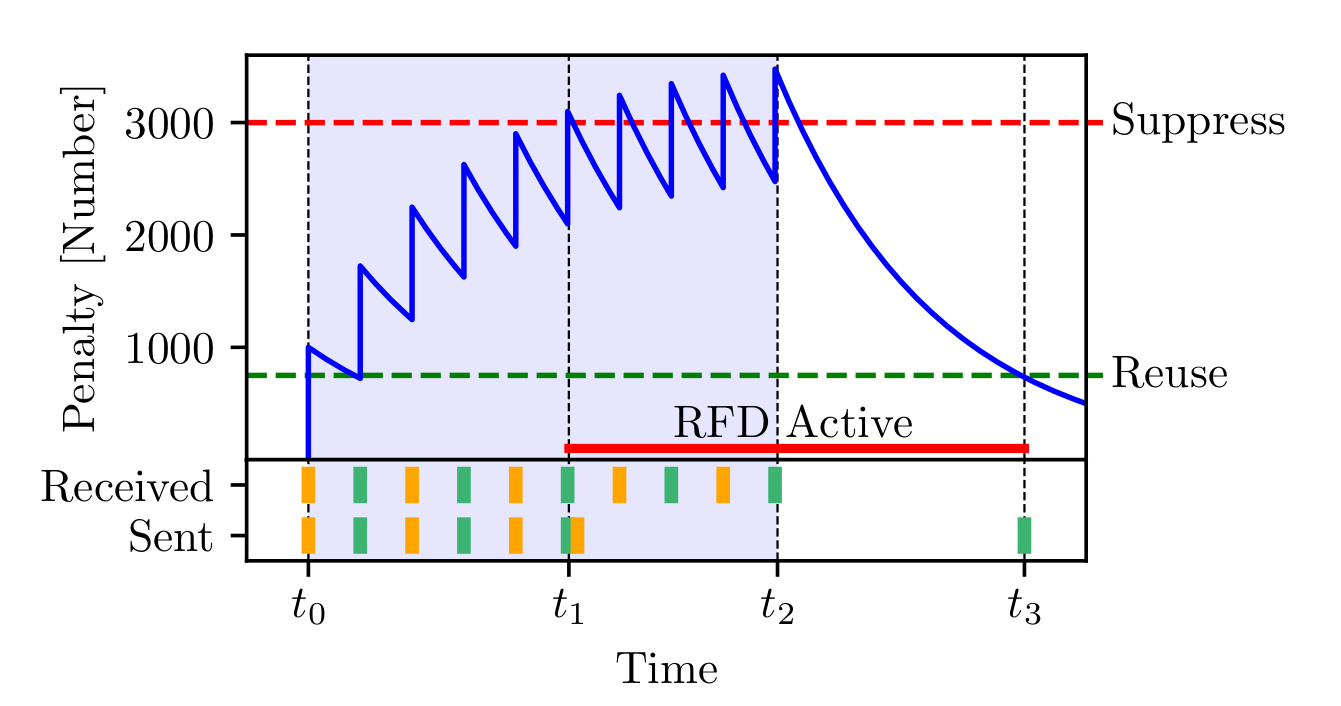
\includegraphics[scale=0.22]{images/RFD/evolution.png}
	\caption{Example of evolution of the \ac{RFD} \textit{figure of merit} taken 
	from \cite{gray2020bgp}, yellow messages represent withdraws and green ones
	are advertisement, dashed lines are the suppression and reuse threshold}
    \label{fig:figure_of_merit}
\end{figure}

\Cref{fig:figure_of_merit} shows an hipotetic evolution of the \ac{RFD} filter,
it doesn't relay on the default value of the cisco implementation.
Is possible to see in the lower part of the plot the messages received by the
\ac{BGP} speaker, yellow one represent withdraws while the green are announcements.
Is possible to see that the penalty value grows at each flaps and as soon it reaches
the suppression threshold the route will not be advertised to any neighbour.
While after the decay has reached the reuse level is possible to advertise the
route again.

Is possible to see that \ac{RFD} doesn't make any difference on its own on what
is causing the flaps, it simply reacts to the actual situation of the network.
Is not even possible to determine where is located the flap, if is the source
that is flapping havily for some reasons or an \ac{AS} in the middle of the
path that is malfunctioning.

\ac{RFD} has a troubled history, maybe even more than \ac{MRAI}.
In \num{2006}, thanks to the pubblication of \cite{mao2002route}, RIPE-378
\cite{smith2006ripe} recomends to disable it.
Few years later the pubblication of the article from Pelsser et al. \cite{pelsser2011route}
RIPE and IETF shares that says that now \ac{RFD} should be used with the updated
parameters \cite{bush2013ripe,rfc7196}.
Unfurtunatly, the study from Gray et al. \cite{gray2020bgp} in \num{2020} shows
that the majority of the \ac{AS} uses \ac{RFD} with
outdated parameters from the \ac{RFC} {2439}.

\fxfatal{Add an end}

%\begin{itemize}
%    \item What is RFD?
%	\item Remember that RFD purpose is to avoid the noise produced
%		by route flapping
%	\item RFD cant distinguish the noise, is to restrictive, R bush point to
%		avoid the use of RFD for the first noise increasing the threshold.
%    \item Why is used RFD?
%    \item Evolution of RFD?
%    \item RFD Today
%\end{itemize}

\section{Topologies}
\label{sec:topologies}

\fxfatal{Talk about the underlaing topology of \ac{BGP} nodes that is not the actual
geographical topology}

The study of the tomografy of the internet has been a really \q{hot} topic in the
90's.
Is not possible to know exactly the Internet network, thats because the edges
of the network are defined by commercial contracts between the nodes that are 
kept private between the parts.

We are not compleatly blind, we know some properities of the network.
Internet is a hierarchical topology where there
are different layers of nodes interconnected one anothere and different types of
nodes.
The nodes in the highest level, Tier one nodes, are the nodes that interconnect
all the lower layers of the network and them are
connected one another in a clique network.

